\documentclass[12pt,oneside]{article}
\usepackage[utf8]{inputenc}
\usepackage{float}
\usepackage[bottom]{footmisc}
\usepackage{bookmark}
\usepackage{microtype}
\usepackage{amsmath}
\usepackage{multicol}
\usepackage{mdframed}
\usepackage{setspace}
\usepackage{pgfplots}
\usepackage{graphicx}
\usepackage{fancyvrb}
\usepackage[absolute]{textpos}\TPGrid{16}{16}
\usepackage{tikz}
  \usetikzlibrary{shapes}
  \usetikzlibrary{arrows.meta}
  \usetikzlibrary{arrows}
  \usetikzlibrary{shadows}
  \usetikzlibrary{trees}
  \usetikzlibrary{fit}
  \usetikzlibrary{calc}
  \usetikzlibrary{positioning}
  \usetikzlibrary{decorations.pathmorphing}
\usepackage{./tikz-uml}
\usepackage{everypage}
  \AddEverypageHook{
    \begin{textblock}{0.5}[0,0](0,0)
      \tikz \node[fill=myred,minimum width=0.5\TPHorizModule,minimum height=16\TPVertModule] {};
    \end{textblock}
    \begin{textblock}{0.125}[0,0](0.5,0)
      \tikz \node[fill=myblack,inner sep=0, minimum width=0.125\TPHorizModule,minimum height=16\TPVertModule] {};
    \end{textblock}
  }
\usepackage{xcolor}
  \definecolor{firebrick}{HTML}{B22222}
  \definecolor{myred}{HTML}{CF0A2C}
  \definecolor{myblack}{HTML}{232527}
\newcommand\dd[1]{\colorbox{gray!30}{\texttt{#1}}}
\usepackage{hyperref}
  \hypersetup{colorlinks=true,allcolors=blue!40!black}
\setlength{\topskip}{6pt}
\setlength{\parindent}{0pt} % indent first line
\setlength{\parskip}{6pt} % before par
% \let\oldsection\section\renewcommand\section{\newpage\oldsection}
\date{\small\today}
\title{%
  Binary Repository Manager\\
  \colorbox{firebrick}{\small\sffamily\color{white}{White Paper}}}
\usepackage[style=authoryear,sorting=nyt,backend=biber,
  hyperref=true,abbreviate=true,
  maxcitenames=1,maxbibnames=1]{biblatex}
  \renewbibmacro{in:}{}
  \addbibresource{books.bib}
\tikzset{node distance=1.6cm, auto, every text node part/.style={align=center, font={\sffamily\small}}}
\tikzstyle{block} = [draw=myblack, fill=white, inner sep=0.3cm, outer sep=0.1cm, thick]
\tikzstyle{ln} = [draw, ->, very thick, arrows={-triangle 90}, every text node part/.append style={font={\sffamily\scriptsize}}]
\begin{document}
\raggedbottom

\maketitle
\begin{abstract}
A software project of almost any size needs to keep its binary artifacts
in a repository, to enable access to them by programmers, tools, and other teams.
The quality of the software that manages the repository matters. There are
a few categories of such a software, which have their
pros and cons, currently on the market. However, none of them fully satisfy
the requirements of a large group of software companies.
That's why a new product is being created.
\end{abstract}

% \onehalfspace

\section{Introduction}

\href{https://en.wikipedia.org/wiki/Binary_repository_manager}{Binary Repository Manager}
(BRM), according to Wikipedia, is ``a software tool designed to optimize the download and storage of
binary files used and produced in software development,'' for example
\dd{.jar} or \dd{.zip} archives. BRM is a critical component of
most \href{https://en.wikipedia.org/wiki/DevOps_toolchain}{DevOps toolchains}~\parencite{erich2018},
residing right after the build pipeline, which is why it is sometimes
called ``build repository'', ``artifact repository'', or ``pipeline state repository''~\parencite{bass15}.

A traditional DevOps pipeline, as explained by~\textcite{humble2010}, expects
the source code to be validated, tested, packaged and versioned automatically
into an \emph{artifact} (a binary file).
Then, the artifact must be stored outside of the source
code repository and become available for later stages of the continuous
delivery pipeline. The BRM is supposed to host these artifacts,
being ``a central point for management of binaries and dependencies,
and an integrated depot for build promotions of internally developed software,''
as noted by~\textcite{davis2016}.

\begin{figure}[H]
\centering
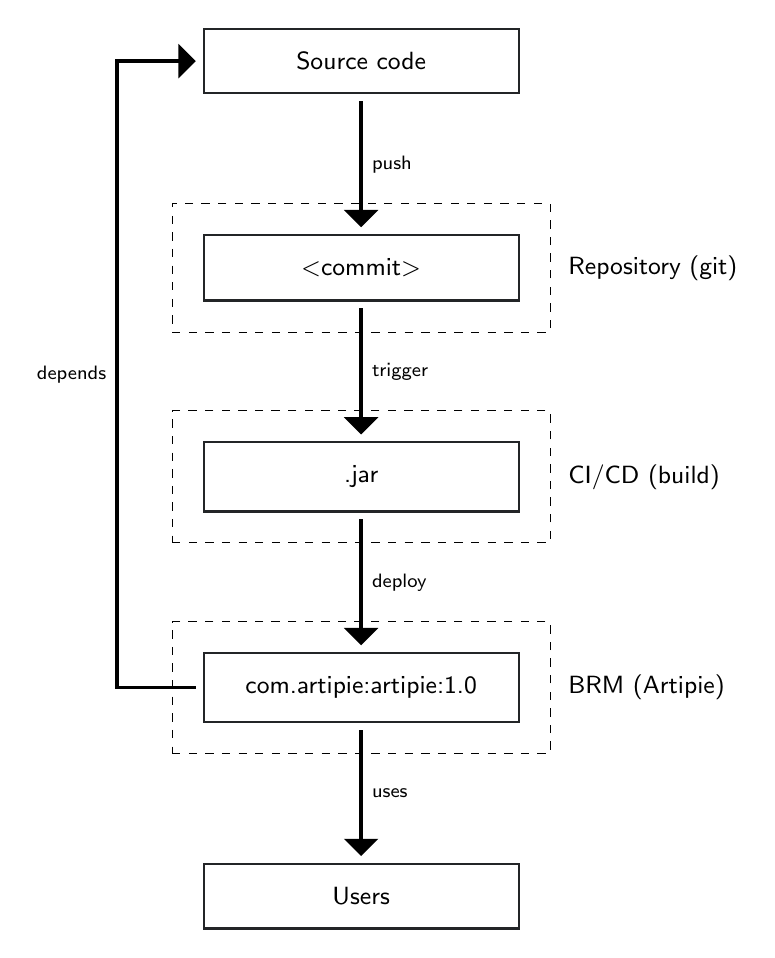
\begin{tikzpicture}
  \node[block, minimum width=4cm] (src) {Source code};
  \node[block, below=of src, minimum width=4cm] (commit) {\textless commit\textgreater};
  \node[fit=(commit), draw, dashed, inner sep=0.3cm, label={[label distance=0.1cm]0:Repository (git)}] (repo) {};
  \node[block, below=of commit, minimum width=4cm] (build) {.jar};
  \node[fit=(build), draw, dashed, inner sep=0.3cm, label={[label distance=0.1cm]0:CI/CD (build)}] (cicd) {};
  \node[block, below=of build, minimum width=4cm] (artifact) {com.artipie:artipie:1.0};
  \node[fit=(artifact), draw, dashed, inner sep=0.3cm, label={[label distance=0.1cm]0:BRM (Artipie)}] (brm) {};
  \node[block, below=of artifact, minimum width=4cm] (users) {Users};
  \path[ln] (src) edge node {push} (commit);
  \path[ln] (commit) edge node {trigger} (build);
  \path[ln] (build) edge node {deploy} (artifact);
  \draw[ln] (artifact.west) -- ([xshift=-10mm]artifact.west) -- node[left] {depends} ([xshift=-10mm]src.west) -- (src.west);
  \draw[ln] (artifact.south) -- node[right] {uses} (users);
\end{tikzpicture}
\caption{The deliver pipeline of an average software development team.}
\label{fig:map}
\end{figure}

The Section~\ref{sec:requirements} lists a few categories of existing
BRM solutions, analyses requirements their customers may have, and emphasize
the most important functional features and non-functional requirements.

\section{Requirements}
\label{sec:requirements}

All existing BRM solutions can be categorized as
public, commercial, hosted, open source, or surrogate.
Even though each of
them partially satisfy the needs of a professional software team, neither
one is perfect.

\begin{description}
  \item[Public]
  There are a few hosted BRMs for different programming languages, like
  \href{https://search.maven.org/}{Maven Central} for Java or
  \href{https://www.rubygems.org}{Rubygems} for Ruby, which are free to use,
  but do not allow private accounts. This means that all artifacts deployed
  by some user become available for all other users. This business model is
  acceptable for open source projects, but is not suitable for software teams
  that develop proprietary software products.

  \item[Commercial]
  There are a few BRMs, like
  \href{https://jfrog.com/artifactory/}{Artifactory}/\href{https://jfrog.com/bintray/}{Bintray}
  of \href{https://jfrog.com}{JFrog}
  and \href{https://www.sonatype.com/nexus-repository-oss}{Nexus}
  of \href{https://www.sonatype.com/}{Sonatype},
  which provide most of the features required by software teams, including
  fine-grained access control, versioning, seamless integration with build
  automation software, and many more. However, these tools are pretty expensive\footnote{%
    The annual cost of a license for a mid-size team of 50-100 developers is:
    \href{https://jfrog.com/pricing/}{around} \$30,000 for Artifactory
    and
    \href{https://www.sonatype.com/product-pricing}{around} \$50,000 for Nexus.
    There are less expensive products too:
    \href{https://inedo.com/proget/pricing}{ProGet} for \$10,000,
  }
  and require certain skills to install and manage them. Moreover, their
  authors (including JFrog and Sonatype) are US-based companies, who may be
  restricted to sell their products to software teams from certain ``sanctioned'' countries\footnote{%
    \href{https://techcrunch.com/2019/07/29/github-ban-sanctioned-countries/}{29th of July, 2019}:
    GitHub, the world's largest host of source code, is preventing users in Iran, Syria, Crimea.
    \href{https://techcrunch.com/2018/12/22/slack-says-it-will-comply-with-sanctions/}{22nd of December, 2018}:
    Slack confirms it will now block all activity in Iran and other sanctioned countries.
  }.

  \item[Hosted]
  There are a few BRMs, which maintain artifacts on their servers,
  like \href{https://www.cloudrepo.io/pricing.html}{CloudRepo} for Java
  or \href{https://pydist.com/}{PyDist} for Python.
  Some BRM creators, like JFrog, provide their products in hosted versions too.
  However, some software teams may not find this option acceptable
  due to security reasons---eventually the data may be lost, if the company
  gets out of the market\footnote{%
    \href{https://www.theverge.com/2015/3/13/8206903/google-code-is-closing-down-github-bitbucket}{13th of March, 2015}:
    Google Code, one of the largest source code repository managers, closed its doors.
  }
  or due to sanctions.

  \item[Open source]
  There are also a few entirely free and open source products, like
  \href{https://archiva.apache.org/index.cgi}{Archiva}, which software
  teams must install, configure and use on their own risk. Even though
  this may sounds like a good solution for a small team, it may not be
  acceptable for a larger group of software developers, who expect their
  artifact repository to be reliable and available.

  \item[Surrogate]
  It is possible to organize a BRM without any software,
  \href{https://www.yegor256.com/2015/09/07/maven-repository-amazon-s3.html}{for example},
  on top of \href{https://aws.amazon.com/s3/}{Amazon S3}
  or a simple FTP server. With the right plugin
  Maven can deploy to Amazon S3 and then fetch artifacts from there
  via their built-in HTTP interface. However, such a solution gives
  very little or no control for a DevOps person and may only
  work for rather small software teams.
\end{description}

\subsection{Features}
\label{sec:features}

There are many important qualities and features software developers and DevOps
engineers expect a BRM to have, in order to be useful in a continuous
delivery pipeline. The most critical
\href{https://en.wikipedia.org/wiki/Non-functional_requirement}{non-functional requirements}
are:

\begin{description}
  \item[Integrability]
  There are plenty of build automation tools for each programming language,
  like \href{https://maven.apache.org/}{Maven} for Java,
  \href{https://www.npmjs.com/}{Npm} for JavaScript, or
  \href{https://github.com/ruby/rake}{Rake} for Ruby.
  There are also many continuous integration tools, like
  \href{https://jenkins.io/}{Jenkins} or \href{https://travis-ci.org/}{Travis}.
  Since automation is the most important aspect of DevOps, as noted by~\textcite{kerzazi2016},
  it is expected to have plugins for each or most of them, to enable seamless
  intregration with the BRM.

  \item[Availability]
  Artifacts are important components of a software development process
  and they must be available right when they are needed by a programmer
  or a build tool, without even small delays and delivered at the highest
  possible speed.

  \item[Scalability]
  Most build artifacts are large binary files. Some of them may even
  be larger than 1Gb, for example \href{https://www.docker.com/}{Docker}
  images or \dd{.war} production-ready Java archives.
  The BRM must be able to maintain large data sets, up to almost no limits.

  \item[Extensibility]
  It is highly desireable to have full access to the source code of the
  BRM and to have an ability to extend it with new plugins and modules. Moreover,
  vendor independence is important.

  \item[Reliability]
  An ability to corrupt the data due to software or harware failures must be
  eliminated, as much as it is possible.
\end{description}

\subsection{Non-functional Requirements}
\label{sec:nfr}

The most important \href{https://en.wikipedia.org/wiki/Functional_requirement}{functional requirements} are:

\begin{description}
  \item[Versions and Tags]
  New artifacts must not replace previously deployed ones.
  Instead, older versions must always be accessible. However,
  it is not expected that the BRM would assign version tags automatically,
  this is done at the pipeline's side.

  \item[Access Control]
  Larger teams may need to control who is allowed to use certain artifacts.
  Moreover, such teams may need to require the integration of authentication
  mechanisms of the BRM with the existing enterprise access-control system,
  via \href{https://en.wikipedia.org/wiki/Lightweight_Directory_Access_Protocol}{LDAP},
  for example. On top of regular access control, encryption mechanisms must
  be in place in order to prevent data leakage in case of software/hardware
  failures or human mistakes, as noted by~\textcite{paule2018}.

  \item[Analytics]
  Traceability between software artifacts is considered a very
  important factor in today development process, as noted by~\textcite{palihawadana2017}.
  BRM must make it possible to visualize dependencies between artifacts and
  operate on them.
\end{description}

There are many other essential features required, including
authentication and authorization, deployment, publishing,
download, removal, usage tracking, email notifications, mirroring,
and so on.

\subsection{Compare with existing solutions}
\label{ref:comparation}

\begin{tabular}{| l | p{3cm} | p{3cm} | p{3cm} |}
\hline
  Feature & Artipie & Artifactory & Nexus \\
  \hline
  Cloud storage providers & S3 based API clouds & AWS S3, Google Cloud, Azure & No \\
  \hline
  Supported repository type
  & Maven, RPM, NPM, Docker, NuGet, PHP-composer, binary files, PyPi, Go, Gem
  & Bower, Chef, CocoaPods, Conan, Conda, CRAN, Debian, Docker, Git LFS, Go, Helm, Maven, NPM, NuGet, Opkg, P2, PHP-composer, Puppet, PyPi, RPM, Gem, SBT, Vagrant, VCS
  & Bower, Docker, NPM, PyPI, Raw, RubyGems, Yum* \\
  \hline
  Installation and maintainance
  & Easy to install via Docker image or to cluster
  & Can be installed locally, but require a team of system administrators to support the cluster
  & Same as Artifactory \\
  \hline
  Performance & TODO & TODO & TODO \\
  \hline
\end{tabular}

* Nexus can uses external plugins to support more repository types

\subsection{Expected Metrics}
\label{ref:metrics}

In a large enterprise it is expected to have the following
numbers, in terms of load, size, and speed:

\begin{tabular}{ll}
Users, total & 80K \\
Artifacts hosted & 100M \\
New artifacts uploaded, daily & 10K \\
Data hosted & 100Tb \\
Data uploaded, daily & 10Gb \\
Concurrent connections, peek & 10K \\
Upload bandwidth, peek & 10M/s \\
Download bandwidth, peek & 100M/s \\
\end{tabular}

Smaller companies may have lower expectations.

\section{Architecture}

Architecure is consisted of 4 essential parts:

\begin{enumerate}
	\item Artipie HTTP engine
        \item Authorization and authentication layer
	\item Repositories
	\item Storage
\end{enumerate}
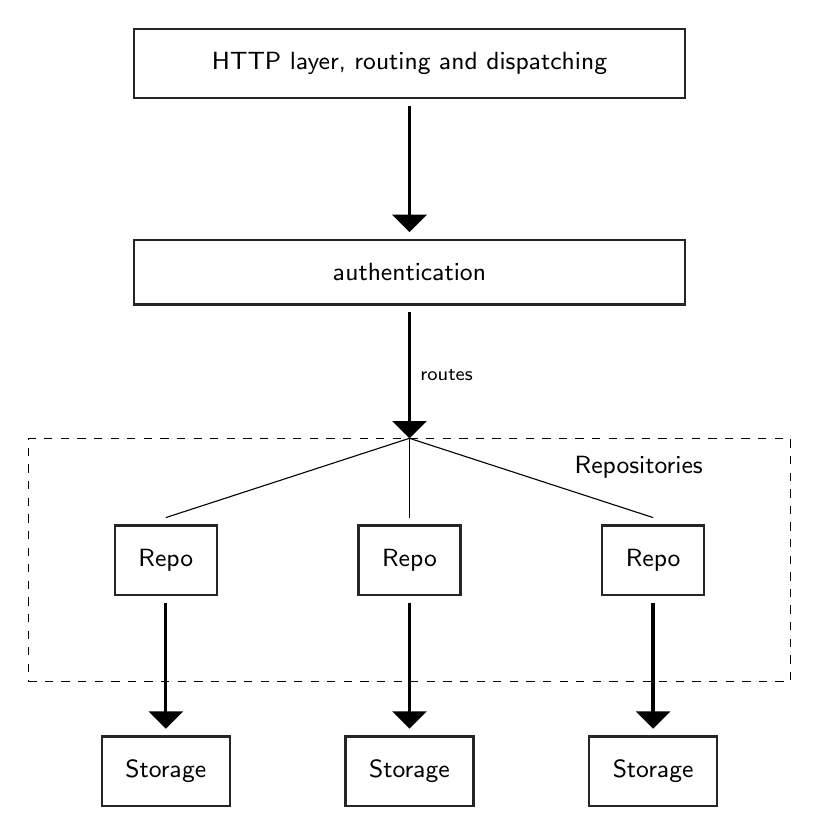
\begin{tikzpicture}
  \node[block] (repo-2) {Repo};
  \node[block, left=of repo-2] (repo-1) {Repo};
  \node[block, right=of repo-2] (repo-3) {Repo};
  \node[fit=(repo-1)(repo-2)(repo-3), draw, dashed, inner sep=1cm, label={[right=10cm, below=0.1cm]1cm:Repositories}] (repos) {};
  \node[block, above=of repos, minimum width=7cm] (auth) {authentication};
  \node[block, above=of auth, minimum width=7cm] (http) {HTTP layer, routing and dispatching};
  \node[block, below=of repo-1] (storage-1) {Storage};
  \node[block, below=of repo-2] (storage-2) {Storage};
  \node[block, below=of repo-3] (storage-3) {Storage};
  \path[ln] (repo-1) -- (storage-1);
  \path[ln] (repo-2) -- (storage-2);
  \path[ln] (repo-3) -- (storage-3);
  \path[ln] (http) -- (auth);
  \path[ln] (auth) edge node {routes} (repos);
  \draw (repos.north) -- (repo-1.north);
  \draw (repos.north) -- (repo-2.north);
  \draw (repos.north) -- (repo-3.north);
\end{tikzpicture}

\subsection{Design considerations}

All of the Artipie components are based on reactive, asynchronous, non-blockng
and back-pressured streams and asynchronous, reactive and non-blocking 
programming principles, allowing Artipie to withstand heavy workloads with a small
amount of kernel threads.

\subsection{Artipie engine}
\label{sec:arti-engine}
Artipie engine is a Java application, which exposes an HTTP endpoint for repository access and management operations.
It routes HTTP requests to repositories and provide authentication mechanisms for repositories.
Each repository encapsulates storage API to access binary blobs and metadata files.

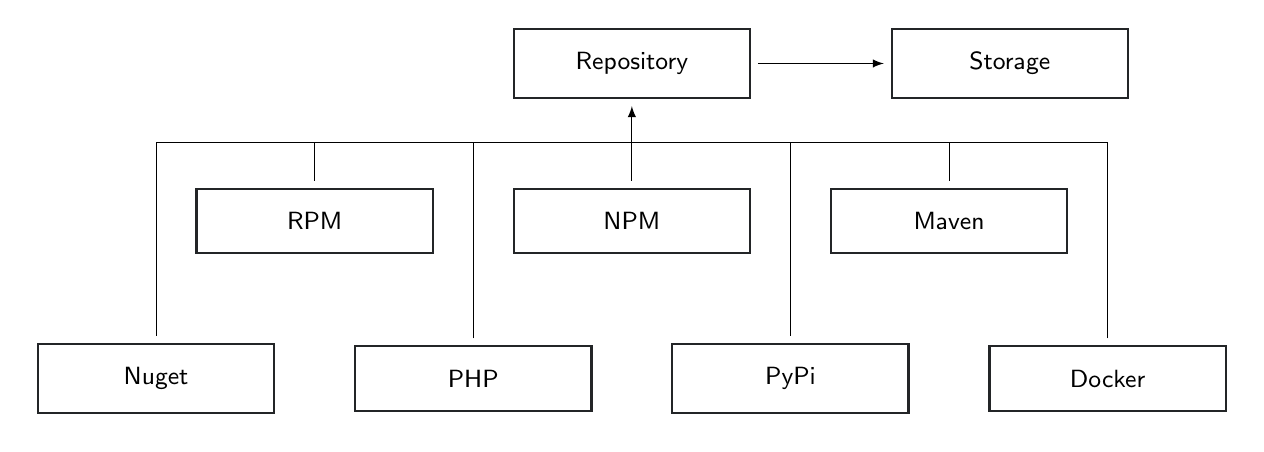
\begin{tikzpicture}[]
  \node[block, minimum width=3cm] (repo) {Repository};
  \node[block, minimum width=3cm, right=of repo] (storage) {Storage};
  \matrix[row sep=10mm, column sep=10mm, yshift=-2cm]{
    \node[block, minimum width=3cm] (rpm) {RPM}; &
    \node[block, minimum width=3cm] (npm) {NPM}; &
    \node[block, minimum width=3cm] (maven) {Maven}; \\
  };
  \matrix[row sep=10mm, column sep=10mm, yshift=-4cm]{
    \node[block, minimum width=3cm] (nuget) {Nuget}; &
    \node[block, minimum width=3cm] (composer) {PHP}; &
    \node[block, minimum width=3cm] (pypi) {PyPi}; &
    \node[block, minimum width=3cm] (docker) {Docker}; \\
  };
  \draw[-latex] (repo) -- (storage);
  \draw[-latex] (npm.north) -- (repo.south);
  \draw (rpm.north) |- (270:10mm) -| ([yshift=-1pt]repo.south);
  \draw (maven.north) |- (270:10mm) -| ([yshift=-1pt]repo.south);
  \draw (nuget.north) |- (270:10mm) -| ([yshift=-1pt]repo.south);
  \draw (composer.north) |- (270:10mm) -| ([yshift=-1pt]repo.south);
  \draw (pypi.north) |- (270:10mm) -| ([yshift=-1pt]repo.south);
  \draw (docker.north) |- (270:10mm) -| ([yshift=-1pt]repo.south);
\end{tikzpicture}

There are various storage implementations, such as:
\begin{enumerate}
    \item File system storage
    \item S3 based storage
    \item In-memory storage
\end{enumerate}

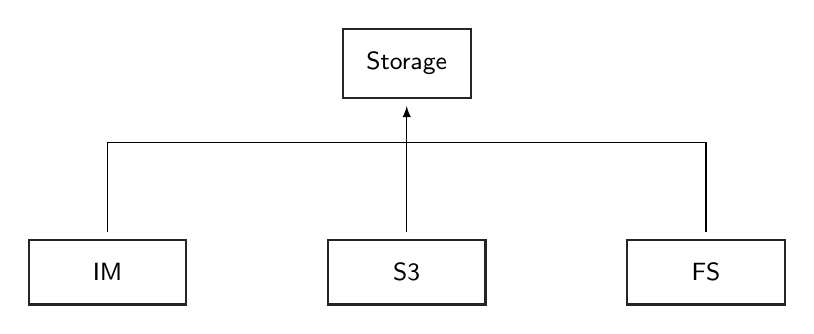
\begin{tikzpicture}[]
  \node[block] (storage) {Storage};
  \node[block, minimum width=2cm, below=of storage] (s3) {S3};
  \node[block, minimum width=2cm, right=of s3] (fs) {FS};
  \node[block, minimum width=2cm, left=of s3] (im) {IM};
  \draw[-latex] (s3.north) -- (storage.south);
  \draw (fs.north) |- (270:10mm) -| ([yshift=-1pt]storage.south);
  \draw (im.north) |- (270:10mm) -| ([yshift=-1pt]storage.south);
\end{tikzpicture}


The common data flow for Artipie upload: client is sending some binary artifact
to the server, server find responsible repository to process the request,
repository is saving the stream to the storage, and after complete it updates metadata
of the repository (it's most common scenario, some repositories works differently,
e.g Docker uses metadata as path).


\begin{center}
\begin{tikzpicture}
\begin{umlseqdiag}
\umlactor[class=Client]{mvn}
\umlobject[class=Server]{Artipie}
\umlobject[class=Repo]{Maven}
\umlobject[class=Storage]{S3}

\begin{umlcall}[op={mvn:deploy}, type=synchron, return={200 OK}]{mvn}{Artipie}
  \begin{umlcall}[op={request}, type=synchron, return={response}]{Artipie}{Maven}
    \begin{umlcall}[op={upload}, type=asynchron, return={complete}]{Maven}{S3}
    \end{umlcall}
    \begin{umlcall}[op={update metadata}, type=asynchron, return={complete}]{Maven}{S3}
    \end{umlcall}
  \end{umlcall}
\end{umlcall}

\end{umlseqdiag}
\end{tikzpicture}
\end{center}

Engine store repository configuration in a .yml file. An example:
\begin{Verbatim}[tabsize=2]
repo:
  type: maven
  storage:
    type: s3
    url: s3://acme.com/snapshot
    username: admin
    password: 123qwe
\end{Verbatim}

This configuration file says that it has a type of maven repository,
which automatically enable maven specific metadata generation logic.
Diving into storage section, artipie asked to use S3 object storage 
as a storage for uploaded artifacts and generated metadata.

The ability to chose where to store artifact gave us the flexibility of choice.
We can choose any type of storage, whether it is a server file system,
an object storage, or a key-value database.
The only requirement is: \hyperref[sec:asto]{Abstract storage} should support it.

Aside from repository configuration, the way artipie stores its settings
also can be customized via artipie.yml file:
\begin{Verbatim}[tabsize=2]
meta:
  storage:
    type: fs
    path: /artipie/storage
\end{Verbatim}
Artipie will resolve this file, and use local filesystem folder for repository settings management. 

\subsection{Repository adapters}
Repository adapters are independent projects, 
aimed to implement meta information generation
layers for a specific package type(npm, maven, etc...).
\hyperref[sec:arti-engine]{Artipie engine} utilizes adapters in order to provide BRM functionality.

Existed adapters:
\begin{itemize}
	\item RPM - \href{https://github.com/artipie/rpm-adapter}{artipie/rpm-adapter}
	\item NPM - \href{https://github.com/artipie/npm-adapter}{artipie/npm-adapter}
	\item Go - \href{https://github.com/artipie/go-adapter}{artipie/go-adapter}
	\item Docker - \href{https://github.com/artipie/docker-adapter}{artipie/docker-adapter}
	\item Maven - \href{https://github.com/artipie/maven-adapter}{artipie/maven-adapter}
	\item Gem - \href{https://github.com/artipie/gem-adapter}{artipie/gem-adapter}
\end{itemize}

\subsection{Abstract storage}
\label{sec:asto}
Abstract storage(asto) is an abstraction over physical data storage system.
It has a simple interface consisted of two operations: put and get.
The simplicity makes it easy to implement the interface of almost any data storage system.

Those design requirements were considered as most important for the asto: 
\begin{enumerate}
  \item High performance
  \item Back pressure of data streams on the level of bytes
	\item Constant memory pool per data stream
	\item Pure java interface, without any external dependencies
	\item High operation latency awareness
\end{enumerate}

The following design options has been considered for the interface design implementation:
\begin{itemize}
  \item \dd{java.io.\{In,Out\}putStream}'s based option. 
  \item RxJava 3 based option.
	\item CompletableFuture and Java 9 Flow based option.
\end{itemize}

The \dd{java.io.\{In,Out\}putStream}'s approach has a conceptual drawback: it's blocking nature,
which affects performance by forcing new thread allocation per user connection. And that is
also a reason why any other blocking approach was not considered.

The RxJava 3 option is close to the ideal one, but the negative side is external
dependency exposition: clients are getting bounded to the RxJava primitives. 

Java non-blocking primitives were counted as the most promising
ones, since \dd{CompletableFuture} and \dd{Flow}-based interface can be implemented in a 
high-performance way and with accordance with all the mentioned requirements.

\subsection{Extensions}
to be written...

\section{Conclusion}
\label{sec:conclusion}

To be written...

\subsection{Acknowledgements}
\label{sec:ack}

The document was originally created by Yegor Bugayenko (y00538675).

\printbibliography%
\end{document}
